% 510K benchmark paper -- LaTeX conversion of paper/draft.md (v0.4)
% Uses the official ICLR 2027 style (iclr2027_conference.sty, copied locally).
% Uncomment \iclrfinalcopy for the camera-ready version, but NOT for submission.
\documentclass{article}
\usepackage{iclr2027_conference,times}
\usepackage{amsmath,amssymb}
\usepackage{booktabs}
\usepackage{graphicx}
\usepackage{hyperref}
\usepackage{url}

\newcommand{\cmark}{\ensuremath{\bullet}}
\newcommand{\pmark}{\ensuremath{\circ}}
\newcommand{\hmark}{\ensuremath{\circledcirc}}

\title{510K: A Benchmark for Latent Relationship Inference and
When-to-Cooperate in Multi-Agent RL}
\author{Anonymous Authors}
\date{}

\begin{document}
\maketitle

\begin{abstract}
Multi-agent benchmarks typically hand the agent its social structure: teams are
fixed and known, and only the question of \emph{how} to cooperate remains.
Realistic settings instead require deciding \emph{whether and with whom} to
cooperate, by inferring relationships from observed behaviour. We present
\textbf{510K}, a four-player shedding card game built to make this
latent-relationship inference problem measurable while remaining coupled to
immediate scoring, terminal competition, and partial observability. Team
identity and team size (2v2 vs 1v3) are determined at deal time by a private
red-A distribution and hidden from observations. 510K offers four independently
ablatable modes (SINGLE, STATIC, DYNAMIC, OBVIOUS), a graded information-reveal
dial, Gymnasium and PettingZoo interfaces with action masking, and reference
baselines. We formalize the resulting challenge as a \emph{belief-inference gap}:
the relationship is decodable from public play (probe AUC up to $1.00$;
logically determined for 36--39\% of decisions), yet policies learn to defer
only to a fixed, known partner (deferral asymmetry $+0.38$, $p<10^{-4}$) and do
not condition on a hidden partner ($+0.00$, $p=0.21$) or an explicitly revealed
one ($-0.04$, $p<10^{-4}$), even though the reveal dial is a near-lossless
information channel ($\ge$91\% of ideal mutual information). Structural probes
show that the axes are not separable: scoring and finishing trade off, and the
hidden team leaves most reward variance unattributable. A 1M-step, 5-seed
masked-PPO suite, a recurrent variant, and a MAPPO baseline corroborate the
failure. 510K is
offered as a benchmark for \emph{when-to-cooperate} decisions under coupled
objectives.
\end{abstract}

\section{Introduction}
A central question in multi-agent reinforcement learning (MARL) is how agents
should behave when several objectives interact and part of the task structure is
hidden. Card games are a natural home for this question, yet existing benchmarks
tend to isolate the difficulties one at a time. Dou Dizhu \citep{douzero}
couples competition with \emph{fixed} cooperation and a sparse terminal reward.
Hanabi \citep{hanabi} is purely cooperative, with neither competition nor an
immediate scoring trade-off. Mahjong \citep{suphx} has scoring and partial
observability but no teams. Tichu, Hearts and Spades have scoring and
partnerships, but the partnerships are \emph{fixed and known}. The picture that
emerges is fragmented: we can measure how an algorithm handles scoring, or
hidden information, or cooperation, but not how it handles them
\emph{together}.

This gap matters because in realistic tasks these aspects are not independent:
acting on one changes the value of the others. A coding agent that makes a test
pass now may damage the architecture later; an agent interacting with others
must simultaneously infer who is aligned with it and whether that alignment
persists. Benchmarks built by stacking independent switches cannot expose such
interactions, because their optimal values decompose.

We introduce \textbf{510K}, a four-player shedding card game designed so that
they do not. 510K couples (i) \emph{immediate scoring} (5/10/K cards collected
in won tricks), (ii) a \emph{terminal competitive} objective (finish first),
(iii) \emph{partial observability}, and (iv) \emph{dynamic cooperation}: team
membership is determined at deal time by the private red-A distribution and is
hidden, so ``who should I help?'' becomes a latent-variable inference problem
rather than a given. Crucially, the axes are not stacked but entangled --- a
single play changes the immediate score, the future pattern space, the
information revealed about relationships, and the race to finish. We make this
precise by formalizing coupling as \emph{non-separability} and by giving each
coupling a measurable signature rather than a rhetorical one
(Section~\ref{sec:coupling}).

The environment ships with four controllable modes (SINGLE, STATIC, DYNAMIC,
OBVIOUS) that ablate the cooperation and information axes, a graded
information-reveal dial, Gymnasium and PettingZoo AEC interfaces with built-in
action masking, and a reference baseline suite. On it we report a capability
profile and a behavioural result: policies learn to cooperate with a fixed,
known partner but neither infer a hidden partner nor exploit an explicitly
revealed one --- an information-utilization failure that mirrors the previously
reported IIGC phenomenon \citep{iigc}.

\paragraph{Contributions.}
\begin{enumerate}
\item \textbf{A complete, tested environment.} Gymnasium single-agent and
PettingZoo AEC interfaces with built-in action masking, four controllable modes,
a deterministic rule bot, and 82 passing tests.
\item \textbf{A challenge decomposition and controlled variants} in which
scoring, terminal competition, partial observability, and dynamic cooperation
are independently ablatable.
\item \textbf{A coupling characterization.} We formalize ``coupled, not
stacked'' as non-separability and give measurable structural signatures for the
objective--objective, objective--cooperation, and cooperation--observability
couplings.
\item \textbf{A baseline suite and evaluation protocol.} Masked PPO, recurrent
masked PPO, and independent (shared-policy) PPO, evaluated identically as
player~0 against fixed bots, with masking compliance as a correctness check and
95\% confidence intervals plus significance tests for all comparisons.
\item \textbf{A capability profile and a cooperation-inference result.} At 1M
steps and 5 seeds SINGLE is hardest for every method, team-mode win rates are
inflated by teammate and team-selection effects, and a behavioural probe shows
policies cooperate with a \emph{fixed, known} partner but neither infer nor
exploit a \emph{hidden/revealed} one.
\end{enumerate}

\section{Related Work}
\subsection{Card-game RL toolkits}
RLCard \citep{rlcard} provides many card games behind a common interface and is
the most widely used toolkit in this space; each included game, however,
isolates a subset of challenges, and none exposes a hidden or dynamically
determined team assignment. OpenSpiel \citep{openspiel} offers game-theoretic
tooling over 50+ games, oriented toward solving extensive-form games rather than
RL under sparse rewards. PyTAG \citep{pytag} covers 20+ tabletop games with a
modern API but shallow per-game depth. These toolkits make card games easy to
run; they do not provide a controlled instrument for studying \emph{interactions}
between challenges.

\subsection{Shedding-type and scoring card games}
DouZero \citep{douzero} established that a shedding-type game with a fixed
landlord role and sparse terminal reward is a serious benchmark: ``long horizons
and sparse reward \ldots the only time a nonzero reward is incurred is at the
end of a game.'' 510K keeps that long-horizon, sparse structure and adds two
ingredients: \emph{hidden, deal-time-determined teams} and an
\emph{immediate-scoring} objective that competes with the terminal finish
objective. Tichu, Hearts and Spades have
scoring and partnerships, but those partnerships are fixed and known, so the
relationship itself is never inferred.

\subsection{Cooperative and imperfect-information benchmarks}
The Hanabi Challenge \citep{hanabi} is the canonical cooperative
imperfect-information benchmark --- agents cannot see their own cards --- but it
has no competition and no scoring trade-off. Overcooked-AI \citep{overcooked}
probes ad-hoc human--AI coordination under full observability. Melting Pot
\citep{melting} studies mixed-motive social interaction at a general substrate
level, not within a compact, fully specified decision problem. None of these
supplies a small, ground-truth, trainable instance in which the relationship
between agents must be inferred.

\subsection{Multi-objective and hidden-role settings}
Multi-objective RL and planning methods tackle trade-offs between conflicting
objectives \citep{hayes}; 510K is a card-game instance with exactly two such
objectives (immediate score and terminal finish) whose tension is measurable.
Diplomacy/Cicero \citep{cicero} and hidden-role LLM studies (Avalon, Werewolf)
demonstrate strong interest in relationship inference at a much larger scale,
but they lack a lightweight RL testbed with ground-truth team assignments. 510K
fills that gap: the latent relationship is known to the simulator, so ``did the
agent infer it?'' is directly measurable.

\subsection{Prior results on 510K}
IIGC \citep{iigc} studies a \emph{phenomenon} on this environment: under hidden
team assignment, policy-gradient updates from different relationships cancel in
expectation, producing \emph{deceptive stability} (the policy appears to stop
learning without converging). The present paper is deliberately complementary:
IIGC asks \emph{why} a learner stalls; we characterize the \emph{environment}
and provide the controlled ablations and behavioural probes that make the
phenomenon reproducible and the mechanism studyable.

\subsection{Positioning}
Table~\ref{tab:positioning} compares 510K with the environments above. Only 510K
couples immediate scoring, terminal competition, partial observability,
\emph{hidden dynamic teams}, and controllable ablation in one game. The claim is
about this combination and its controllability, not about being the hardest card
game: each individual challenge is studied elsewhere, and our contribution is to
make them jointly controllable and measurable.

\begin{table}[t]
\centering
\footnotesize
\setlength{\tabcolsep}{3pt}
\caption{Positioning: \cmark{} strong/present, \hmark{} partial, \pmark{} absent.}
\label{tab:positioning}
\begin{tabular}{lccccccc}
\toprule
Challenge & 510K & DouDizhu & Hanabi & Mahjong & Tichu & Overcooked & SMAC \\
\midrule
Immediate scoring & \cmark & \pmark & \pmark & \cmark & \cmark & \pmark & \pmark \\
Terminal competition & \cmark & \cmark & \pmark & \cmark & \cmark & \pmark & \cmark \\
Partial observability & \cmark & \cmark & \cmark & \cmark & \hmark & \pmark & \hmark \\
Team cooperation & \cmark$_{\text{hidden}}$ & \cmark$_{\text{fixed}}$ & \cmark$_{\text{all}}$ & \pmark & \cmark$_{\text{fixed}}$ & \cmark & \hmark \\
\textbf{Hidden/dynamic teams} & \textbf{\cmark} & \pmark & \pmark & \pmark & \pmark & \pmark & \pmark \\
Controlled ablation & \cmark & \pmark & \pmark & \pmark & \pmark & \hmark & \hmark \\
\bottomrule
\end{tabular}
\end{table}

\section{The 510K Environment}
\subsection{Rules}
510K is a shedding-type card game played with a standard 52-card deck (4
players; a 3-player variant with two jokers is also implemented). Each player is
dealt 13 cards. On a turn a player must either play a combination that beats the
current trick or pass; when all other active players pass, the trick ends and
its accumulated \emph{score} is awarded to the trick leader, who opens the next
trick. The result is a deliberately mixed reward structure: a dense, immediately
observable score signal layered on a sparse terminal objective.

\paragraph{Immediate scoring.} Cards score when collected in a won trick:
$5 = 5$ points, $10 = 10$ points, $K = 10$ points. Each trick thus carries an
immediate-score signal that competes with the game-level objective of emptying
one's hand first.

\paragraph{Terminal objective.} The game ends when (SINGLE) the first player
empties their hand, or (team modes) when both members of a team finish. Final
reward combines collected 510K points with finish-position bonuses.

\paragraph{Patterns.} 16 playable combination types: singles, pairs, triples,
three-with-kicker, three-with-pair, straights, consecutive pairs, airplanes
(with/without kickers), bombs, the eponymous \textbf{510K} (5-10-K, suited and
non-suited), joker bomb, and (in team modes) red-A singles/pairs.

\subsection{Team mechanics: hidden dynamic cooperation}
\begin{itemize}
\item \textbf{STATIC}: fixed teams $\{0,2\}$ vs $\{1,3\}$; identities known.
\item \textbf{DYNAMIC}: teams are determined at deal time by the red-A
distribution: any player holding a red ace (or all four aces) joins the ``red''
team. Team membership is \emph{hidden} from observations and must be inferred
from others' play.
\item \textbf{OBVIOUS}: same deal-time teams as DYNAMIC, but the observation
includes a 4-bit team mask --- a direct ablation of teammate-identity
visibility.
\end{itemize}
The hidden relationship can be a 2v2 partnership or a 1v3/3v1 solo
configuration: the red team has size 2 with probability
$1 - 4\binom{50}{11}/\binom{52}{13} \approx 0.765$ and size 1 otherwise --- a
closed-form hypergeometric fact verified exactly (Section~6.9). We treat the
solo case as a feature: the latent variable to infer is not only \emph{who} is
my partner but \emph{whether I even have one}. Because the team is hidden, the
reward function itself is latent: the same observation--action pair can map to
different returns depending on the deal.

\subsection{Interfaces}
\begin{itemize}
\item \textbf{Gymnasium single-agent} (\texttt{FiveTenKEnv}, registered as
\texttt{510K-v0}; \citealp{gymnasium}): controls player 0; other players are
auto-played by a random or rule bot. Observation is a normalized 112-dim vector
(own-hand one-hot + last-trick cards/type + hand sizes + current player + pass
count + own score; +4 team bits in OBVIOUS). 300-discrete action space with
built-in masking; passes \texttt{gymnasium.utils.env\_checker} in all four
modes.
\item \textbf{PettingZoo AEC} (\texttt{FiveTenKMultiEnv}; \citealp{pz}):
controls all players; observation is an \texttt{\{observation, action\_mask\}}
dict per agent; passes the official \texttt{api\_test}. We provide AEC (not
Parallel) because 510K is strictly turn-based with irregular turn order.
\item \textbf{Action masking} is built in; the largest hand produces
$\approx$75 valid patterns, far below the 300 action slots.
\end{itemize}

\subsection{Reproducibility}
Seeded \texttt{reset}, deterministic rules, \texttt{pip install env-510k}, 82
passing tests, and a published reference implementation (\texttt{baselines/}).
A trajectory release and Docker configuration are planned.

\section{Challenge Decomposition and Controlled Variants}
The central design claim: 510K does not \emph{stack} challenges; they
\textbf{interact and alter each other's value}. Playing a 5/10/K card changes
the immediate score, the remaining hand and future pattern space, may reveal or
hide information about team membership, and affects who can finish first. This
yields a difficulty hierarchy: immediate reward $\to$ situation value $\to$
teammate/opponent intent $\to$ future state space $\to$ game outcome.

\subsection{Coupling is non-separability, not stacking}
A benchmark \emph{stacks} challenges when a difficulty (or the optimal value)
decomposes additively across axes. Let the axes be scoring (S), terminal
competition (T), partial observability (P) and hidden cooperation (C). The
couplings we deliberately instantiate are:
\begin{itemize}
\item \textbf{C1 objective entanglement (S$\times$T).} A 5/10/K play moves the
immediate score and the race to finish \emph{in tension}: securing points means
keeping control of the trick, while shedding fast concedes points.
\item \textbf{C2 cooperation $\times$ observability (C$\times$P).} In DYNAMIC
the reward is indexed by the latent team $T$; two histories that look identical
can induce different reward mappings. Partial observability is
\emph{constitutive of} the cooperation structure, not additive noise.
\item \textbf{C3 objective $\times$ cooperation (S$\times$C).} The same scoring
objective has a different payoff depending on team structure.
\item \textbf{C4 information $\times$ cooperation $\times$ state.} The value of
revealing the team depends on whether the agent has a partner (1v3 vs 2v2) and
on the terminal race; \texttt{RevealEnv} turns this into a graded dial.
\end{itemize}
Because every axis is a code-level switch, each coupling has a \emph{measurable}
signature (Section~\ref{sec:coupling}) rather than a rhetorical one.

\paragraph{Controlled variants.}
\begin{table}[t]
\centering
\footnotesize
\caption{Controlled variants (the experimental backbone).}
\label{tab:variants}
\begin{tabular}{lccccc}
\toprule
Axis & SINGLE & STATIC & DYNAMIC & OBVIOUS & Reveal \\
\midrule
Scoring & $\checkmark$ & $\checkmark$ & $\checkmark$ & $\checkmark$ & $\checkmark$ \\
Terminal competition & $\checkmark$ & $\checkmark$ & $\checkmark$ & $\checkmark$ & $\checkmark$ \\
Teams & none & fixed, known & hidden & hidden, revealed & DYNAMIC + frac. \\
Partial observability & $\checkmark$ & $\checkmark$ & $\checkmark$ & $\checkmark$ & graded \\
\bottomrule
\end{tabular}
\end{table}

The information-reveal axis is realized by \texttt{RevealEnv}, which includes
the team mask with probability $p$ per decision ($p{=}0 \equiv$ DYNAMIC,
$p{=}1 \equiv$ OBVIOUS).

\section{Experimental Setup}
\paragraph{Baselines (all action-masked).} \textbf{Masked PPO (MLP)}:
\texttt{sb3\_contrib.MaskablePPO} \citep{sb3} (PPO; \citealp{ppo}) controlling
player~0 against fixed auto-played opponents (random or rule bot).
\textbf{Recurrent PPO (LSTM)}: \texttt{RecurrentPPO} \citep{sb3} + a custom
\texttt{MaskedLstmActorCriticPolicy} (sb3-contrib ships no masked LSTM policy;
we embed the mask in the observation and apply it inside the policy); its
evaluation collapses in DYNAMIC/OBVIOUS (Section~\ref{sec:conditioning} and
Section~\ref{sec:limitations}). \textbf{Independent PPO (IPPO)}: a
shared-policy self-play baseline (\texttt{SelfPlayEnv}): one policy controls all
seats.

\paragraph{Evaluation protocol.} Every policy is evaluated identically: the
trained policy plays player~0 against fixed opponents for seeded games.
Metrics: win rate, mean total reward (mean $\pm$ 95\% CI), mean episode length,
and illegal-action rate (masking compliance).

\paragraph{Protocol.} All runs are 1M steps in modes
SINGLE/STATIC/DYNAMIC/OBVIOUS: masked PPO with 5 seeds, IPPO with 3, recurrent
PPO with 2. Capability-profile analysis asks which method collapses under
(hidden team $\times$ partial observability).

\paragraph{Coupling and cooperation-inference probes.} Structural coupling
signatures are measured with fixed bots driving all four seats
(\texttt{coupling\_probes.py}): a score--finish rank correlation (C1) and a
reward-attribution decomposition (C2/C3). Strategy-level behaviour is probed
with trained policies (\texttt{analyze\_team\_conditioning.py}) via a deferral
asymmetry (Section~\ref{sec:conditioning}).

\paragraph{Statistical analysis.} Cells are reported as mean $\pm$ 95\% CI
(t-based, ddof=1). We use Welch $t$-tests for algorithm comparisons, paired
$t$-tests for within-checkpoint comparisons, a per-seed linear slope of win
rate on reveal probability $p$ with a one-sample $t$-test, and two-proportion
$z$-tests for the deferral asymmetries (\texttt{baselines/stats.py}).

\paragraph{Compute budget.} Measured on a single GPU: MaskablePPO
$\approx$500 env-steps/s ($\approx$40 min per 1M-step run); the 4-mode
$\times$ 5-seed masked-PPO matrix costs $\approx$13 GPU-hours.

\section{Results}
Core results use masked PPO trained for 1M steps with 5 seeds and evaluated as
player~0 against rule bots. All policies have illegal-action rate 0.0 ---
masking is respected exactly.

\subsection{Capability profile across modes and methods}
Win rate (fraction of episodes with positive team reward), mean $\pm$ 95\% CI
(all 1M steps). Recurrent is the \texttt{ent\_coef}=0.05 variant (2 seeds, no
CI).

\begin{table}[t]
\centering
\small
\caption{Capability profile. $^\dagger$Recurrent checkpoints remain
seed-degenerate in DYNAMIC/OBVIOUS.}
\label{tab:capability}
\begin{tabular}{lccc}
\toprule
mode & MLP PPO (5 seeds) & recurrent PPO (2)$^\dagger$ & IPPO (3) \\
\midrule
SINGLE & $0.516 \pm 0.029$ & 0.540 & $0.300 \pm 0.114$ \\
STATIC & $0.774 \pm 0.031$ & 0.735 & $0.737 \pm 0.094$ \\
DYNAMIC & $0.862 \pm 0.016$ & $0.850^\dagger$ & $0.810 \pm 0.025$ \\
OBVIOUS & $0.822 \pm 0.006$ & $0.780^\dagger$ & $0.807 \pm 0.080$ \\
\bottomrule
\end{tabular}
\end{table}

\begin{figure}[t]
\centering
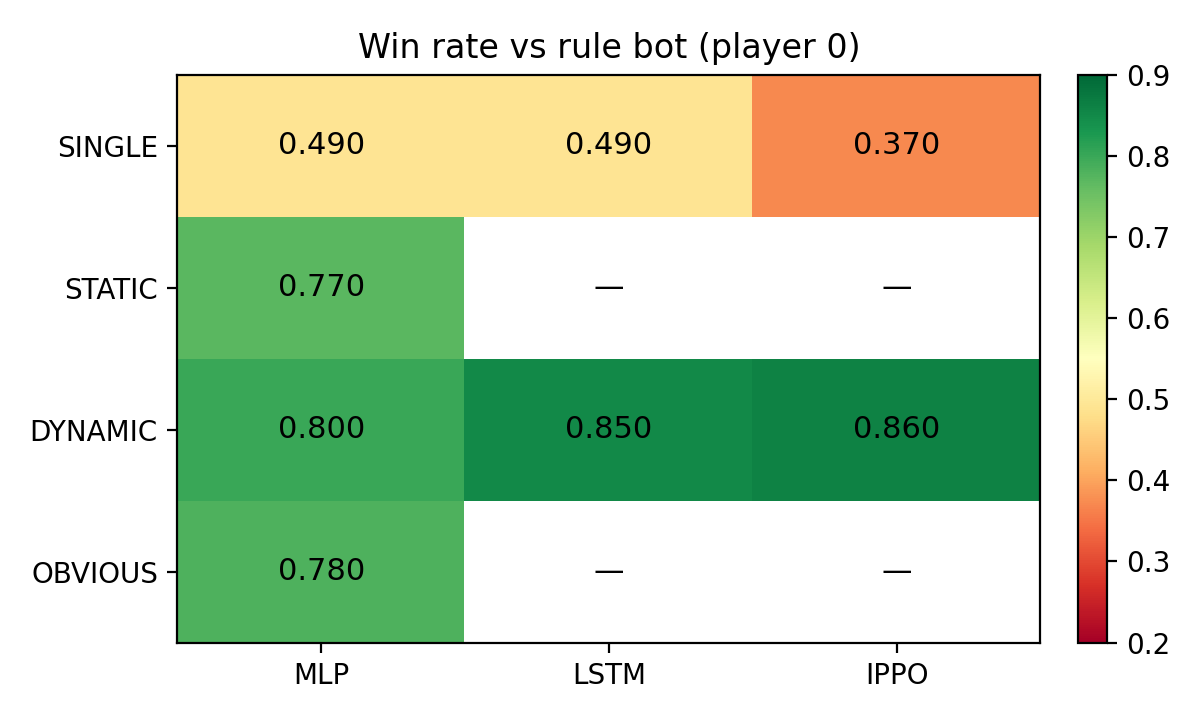
\includegraphics[width=0.42\linewidth]{figs/capability_heatmap.png}
\caption{Capability profile (win rate vs rule bot, player 0).}
\label{fig:heatmap}
\end{figure}

Reading: \textbf{SINGLE is the hardest setting} for every method (MLP
$0.516 \pm 0.029$, IPPO $0.300 \pm 0.114$, below chance). \textbf{MLP > IPPO in
all four modes}, significantly in SINGLE (Welch $p=0.007$) and DYNAMIC
($p=0.001$) but not in STATIC ($p=0.22$) or OBVIOUS ($p=0.50$). Team-mode win
rates are inflated by two effects: a teammate's play contributes to the
outcome, and DYNAMIC/OBVIOUS teams are \emph{selected} by holding a red ace, so
the agent's team tends to hold stronger cards; we therefore treat per-agent and
behavioural metrics as the primary evidence. DYNAMIC is significantly above
OBVIOUS ($0.862$ vs $0.822$, paired $t=8.94$, $p=0.0009$), but the difference is
small and opponent-dependent (it reverses against random bots).

\paragraph{Opponent robustness.} Re-evaluating the same rule-trained
checkpoints against random bots (\texttt{evaluate\_opponents.py}) preserves the
ordering: SINGLE stays hardest (MLP $0.764$, IPPO $0.450$) and MLP > IPPO in
every mode (STATIC $0.950$/$0.867$, DYNAMIC $0.948$/$0.907$, OBVIOUS
$0.958$/$0.950$; full table in Appendix~A). Team modes saturate near ceiling
against random bots, so the rule bot is the more informative opponent.

\subsection{Information-revelation ablation}
Masked PPO with the team revealed with probability $p$ per decision
(\texttt{RevealEnv}), all at 1M steps $\times$ 5 seeds:

\begin{table}[t]
\centering
\small
\caption{Information-reveal dose--response (MLP).}
\label{tab:reveal}
\begin{tabular}{lcc}
\toprule
reveal $p$ & win rate & reward \\
\midrule
0.00 (DYNAMIC) & $0.862 \pm 0.015$ & $78.0 \pm 5.0$ \\
0.25 & $0.838 \pm 0.020$ & $79.3 \pm 4.3$ \\
0.50 & $0.838 \pm 0.019$ & $76.9 \pm 3.4$ \\
0.75 & $0.844 \pm 0.029$ & $77.7 \pm 3.4$ \\
1.00 (OBVIOUS) & $0.822 \pm 0.005$ & $69.6 \pm 0.1$ \\
\bottomrule
\end{tabular}
\end{table}

\begin{figure}[t]
\centering
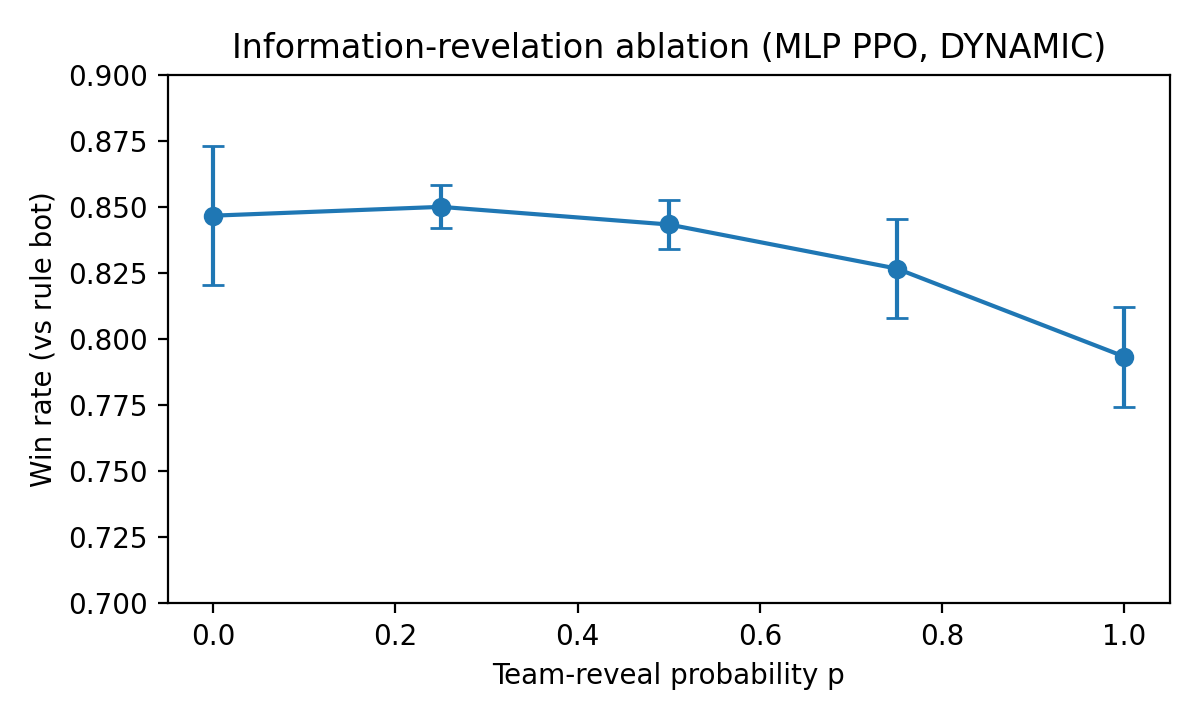
\includegraphics[width=0.42\linewidth]{figs/reveal_curve.png}
\caption{Information-revelation dose--response (MLP, DYNAMIC).}
\label{fig:reveal}
\end{figure}

Against rule-bot opponents the curve is flat to slightly decreasing. A
per-seed linear fit gives a mean slope of $-0.030$ per unit $p$ (one-sample
$t=-6.12$, $p=0.0036$, $n=5$), and the paired $p{=}0$ vs $p{=}1$ difference is
$+0.040$ ($p=0.0009$): at 1M steps, revealing the team significantly
\emph{hurts} rather than helps. Prop.~C shows the dial is a nearly-linear
information channel ($\ge$91\% of the ideal $p\,H(T)$), so this is a genuine
\emph{information-utilization} failure, not an unturned dial. Against random
bots the difference reverses and is within noise, so the opponent-robust claim
is the behavioural one.

\subsection{Structural coupling signatures (C1--C3)}
\label{sec:coupling}
Fixed-bot probes over 500 games/mode. \texttt{top1st} = fraction of games whose
top scorer finishes first (chance 0.25, binomial test); $\rho$ = within-game
rank correlation between score and finish position (mean $\pm$ 95\% CI,
one-sample $t$-test); $dR/d(\text{own})$ = OLS slope of reward on own score;
$R^2$ = reward variance explained by own+teammate scores (bootstrap 95\% CI).

\begin{table}[t]
\centering
\small
\caption{Structural couplings, rule bot (all $\rho<0$ and all top1st $>0.25$ at
$p<10^{-9}$).}
\label{tab:coupling}
\begin{tabular}{lccccc}
\toprule
mode & top1st & $\rho$ (95\% CI) & $dR/d$(own) & corr(own,$R$) & $R^2$ (95\% CI) \\
\midrule
SINGLE & 0.596 & $-0.271 \pm 0.043$ & 1.51 & 0.893 & 0.797 [0.78, 0.82] \\
STATIC & 0.592 & $-0.546 \pm 0.038$ & 2.34 & 0.587 & 0.844 [0.82, 0.87] \\
DYNAMIC & 0.604 & $-0.565 \pm 0.036$ & 2.16 & 0.569 & 0.337 [0.30, 0.37] \\
OBVIOUS & 0.374 & $-0.364 \pm 0.046$ & 2.23 & 0.588 & 0.356 [0.32, 0.39] \\
\bottomrule
\end{tabular}
\end{table}

The random bot shows the same pattern (e.g.\ SINGLE $R^2 = 0.638$ [0.61, 0.66]
vs DYNAMIC $0.200$ [0.17, 0.23]). C1 holds: scoring and finishing first
genuinely trade off. C3 holds: corr(own score, reward) drops from $\approx$0.8
in SINGLE to 0.44--0.59 in team modes. C2 holds: in hidden-team modes only
0.20--0.36 of reward variance is attributable to own+teammate scores, versus
0.64--0.84 in SINGLE/STATIC (non-overlapping bootstrap CIs for SINGLE vs
DYNAMIC).

\subsection{Can a policy condition on the hidden team? (C2/C4)}
\label{sec:conditioning}
On every following decision we measure the deferral asymmetry
$\mathrm{asym} = P(\text{pass} \mid \text{true partner leads}) -
P(\text{pass} \mid \text{opponent leads})$.

\begin{table}[t]
\centering
\small
\caption{Deferral asymmetry; $p$-values are one-sample $t$-tests against zero.}
\label{tab:conditioning}
\begin{tabular}{lcc}
\toprule
mode & MLP (5 seeds) & recurrent e05 (2) \\
\midrule
STATIC & $+0.379$ ($p<10^{-4}$) & $+0.375$ \\
DYNAMIC & $+0.003$ ($p=0.21$) & $-0.043$ \\
OBVIOUS & $-0.037$ ($p<10^{-4}$) & $-0.066$ \\
\bottomrule
\end{tabular}
\end{table}

A fixed, known partner is learned; a hidden partner is not inferred (null); and
merely revealing the partner does not help --- OBVIOUS is significantly
\emph{negative} and its win rate is lower than DYNAMIC. Four of the five
OBVIOUS seeds produce identical decision sequences on the shared evaluation
deals, a signature of a policy that has collapsed to ignoring the team bits.

\paragraph{Recurrent and CTDE corroboration.} The MLP is memoryless, so we also
trained two masked-LSTM variants and a MAPPO baseline with a centralized critic
and self-play (1M steps). The healthiest LSTM is seed-diverse in SINGLE
($0.540 \pm 0.030$) and STATIC and learns fixed-partner cooperation
($+0.37/+0.38$), yet shows no cooperation under hidden or revealed teams
(DYNAMIC $-0.043$; OBVIOUS $-0.07/-0.06$). MAPPO likewise shows no positive
deference to the hidden partner (DYNAMIC asym $-0.021$, range $-0.025$ to
$-0.016$, 3 seeds) despite much higher win rates ($0.93$--$0.98$) --- so the
failure is neither memoryless nor PPO-specific, and team win rate is again a
poor metric.

\subsection{The belief-inference gap}
\label{sec:beliefgap}
We formalize the challenge as a \emph{belief-inference gap}: the latent
relationship $z$ (who, if anyone, is a teammate) must be inferred from the
public history $h_t$, and the policy should condition on it. A linear probe over
the agent's features predicts the true teammate set with AUC $0.60$/$0.91$
(DYNAMIC/OBVIOUS) from a single observation, rising to $0.70$/$1.00$ with
history, and the relation is \emph{logically determined} by public information
for $39\%$/$36\%$ of decisions; yet the trained policy's deferral asymmetry is
$+0.003$ (DYNAMIC, $p=0.21$) and $-0.037$ (OBVIOUS, $p<10^{-4}$). The
relationship is decodable from public play but unused.

\begin{table}[t]
\centering
\small
\caption{Belief-inference gap (1200 games/mode, 13.9k/17.8k agent decisions).}
\label{tab:beliefgap}
\begin{tabular}{lcccc}
\toprule
mode & determinable & obs-probe AUC & hist-probe AUC & policy asym \\
\midrule
DYNAMIC & 0.39 & 0.60 & 0.70 & $+0.003$ \\
OBVIOUS & 0.36 & 0.91 & 1.00 & $-0.037$ \\
\bottomrule
\end{tabular}
\end{table}

\subsection{Hidden-relationship robustness (1v3 vs 2v2)}
DYNAMIC deals split by red-team size (76\% 2v2 / 24\% 1v3). Over the five seeds
the 2v2 and 1v3 win rates are $0.840$ (range $0.82$--$0.85$) and $0.891$
($0.85$--$0.93$); the deal split is $384/116 \approx 76.8\%/23.2\%$, matching
Prop.~A. The results are insensitive to team composition, so conclusions do not
depend on the intentionally unfiltered 1v3 deals.

\subsection{Learning curves}
Per-chunk evaluation history (Figure~\ref{fig:curves}) shows that every mode
plateaus early: the mean slope over the last three chunks is not different from
zero in any mode ($|\text{slope}| \le 0.004$ per 100k steps, all $p>0.24$,
$n=5$ seeds). SINGLE never leaves chance (final $0.516 \pm 0.029$ vs $0.5$,
$p=0.195$); DYNAMIC and OBVIOUS are statistically flat by 300k already (final
$0.862$/$0.822$ vs $0.836$/$0.796$, paired $p=0.13$ and $0.07$). The
information-utilization failure is therefore not a ``not yet trained''
artifact.

\begin{figure}[t]
\centering
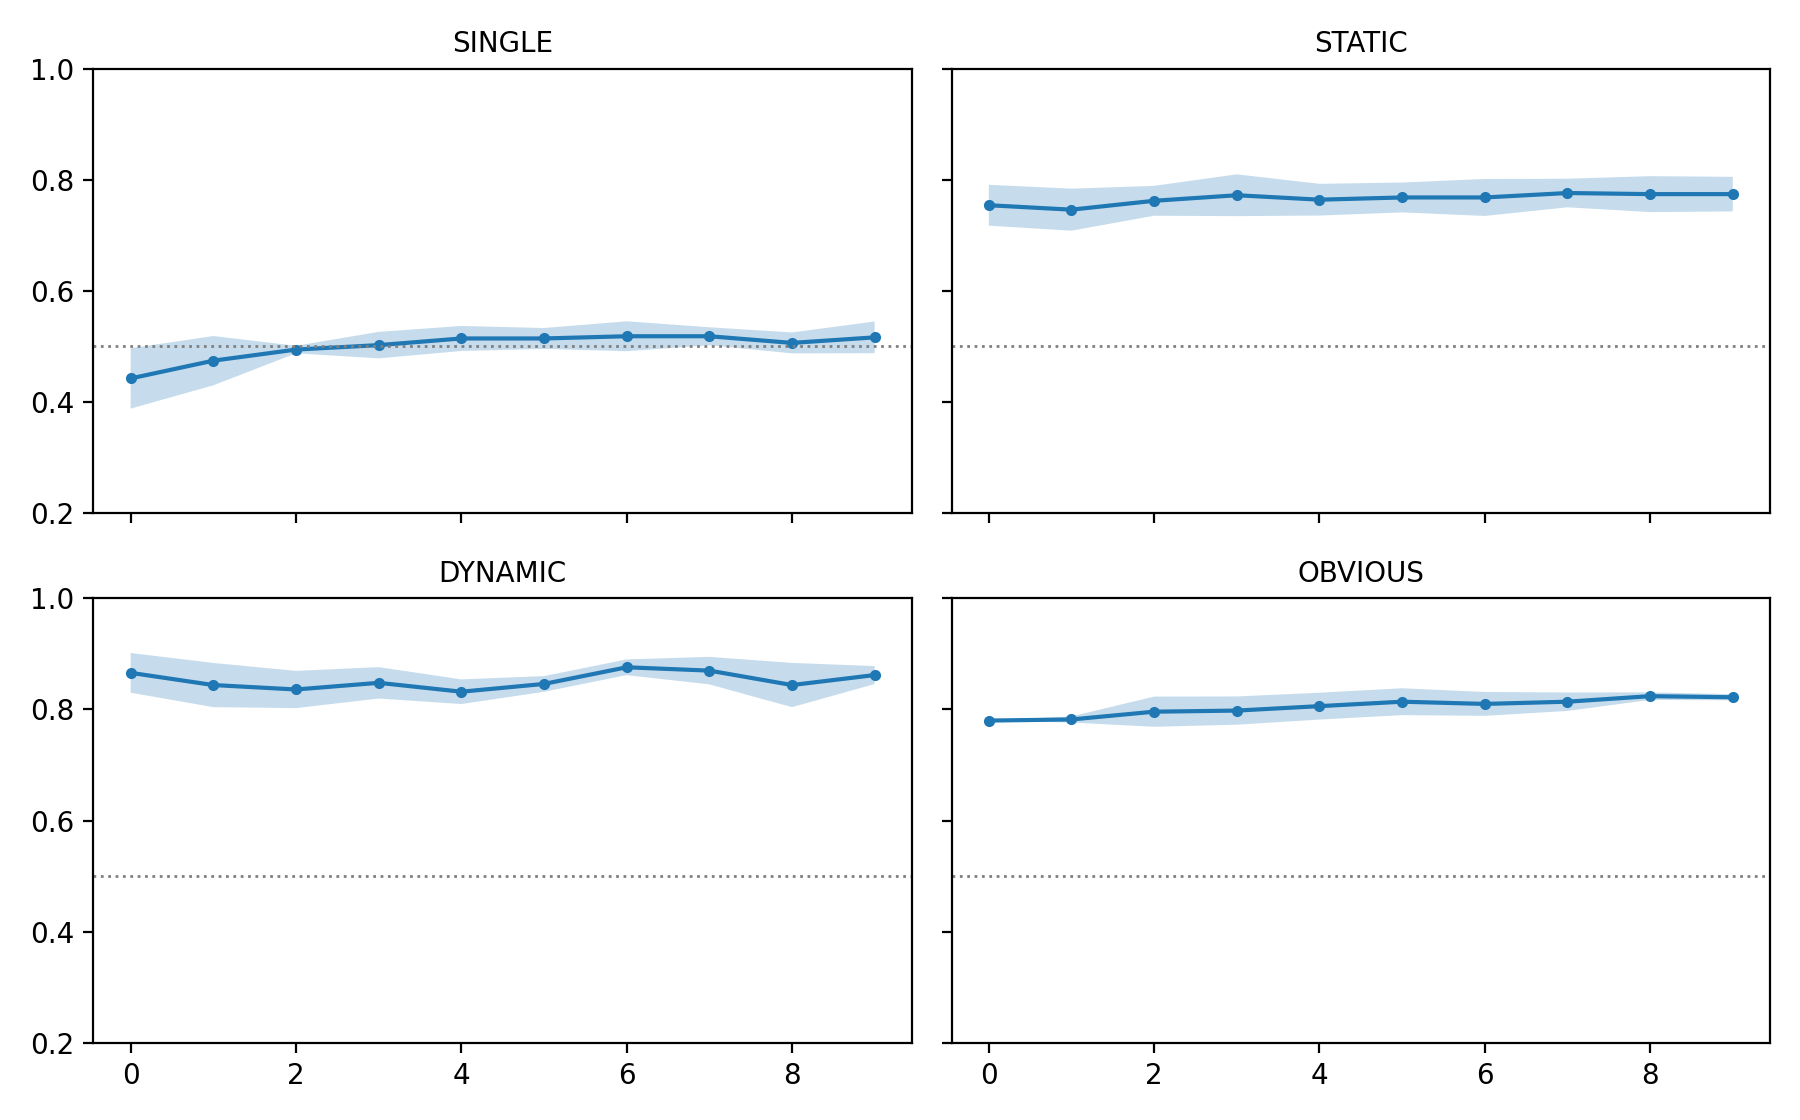
\includegraphics[width=0.45\linewidth]{figs/learning_curves_modes.png}
\caption{Learning curves per mode (MLP, mean $\pm$ 95\% CI over 5 seeds).}
\label{fig:curves}
\end{figure}

\subsection{Connection to IIGC}
Under hidden teams, PPO exhibits \emph{deceptive stability} \citep{iigc}: at 1M
steps its evaluation performance is unchanged whether or not the team is
revealed, and the behavioural probe shows it never conditions on the true
partner --- while the OBVIOUS ablation does not help and slightly hurts. This
benchmark paper supplies the environment characterization behind that
phenomenon.

\subsection{Theoretical grounding}
Four analytical results tie the environment's design and the observed results
together:
\begin{enumerate}
\item \textbf{Team-size prior (design).} The red team has size 2 with
probability $1 - 4\binom{50}{11}/\binom{52}{13} \approx 0.765$ and size 1
otherwise --- a derived hypergeometric fact (verified exactly over 20k deals).
The latent relationship includes both identity and size.
\item \textbf{Membership probabilities.} $P(\text{agent} \in \text{red})
\approx 0.441$, and $P(\text{agent is the solo red player}) \approx 0.059$.
\item \textbf{The reveal dial is a nearly-linear information channel:}
$\mathrm{MI}(p) = p\,H(T) - \delta(p)$, with $\delta(p) = 0$ iff no deal is 1v3;
measured $\mathrm{MI} = 0.62/1.26/1.91$ at $p = 0.25/0.5/0.75$ ($\ge$91\% of
ideal), so the axis \emph{was} swept.
\item \textbf{Reward dilution explains coarse win rates:} team-mode rewards
aggregate two players' scores, and the teammate contributes $\approx$half the
variance (own share $\approx 0.51$), so team win rate is a threshold on a
diluted signal.
\end{enumerate}

\section{Discussion, Limitations, and Future Work}
\label{sec:limitations}
510K is not claimed to be the ``hardest card game''; it is a \emph{controllable
combination} of individually-studied challenges --- a unified testbed rather
than a SOTA chase. Unlike social benchmarks with opaque relationship structure,
it has ground-truth deal-time teams, so ``did the agent infer the
relationship?'' is directly measurable; our deferral asymmetry realizes this and
finds that current PPO does \emph{not} condition on the true partner.

\paragraph{Limitations.}
\begin{itemize}
\item \emph{Coverage.} The masked-PPO matrix and the full reveal curve are
complete at 1M $\times$ 5 seeds and IPPO at 1M $\times$ 3 seeds; the recurrent
baselines cover all modes at 2 seeds but remain partly degenerate, and opponents
are rule/random bots (no self-play or search).
\item \emph{Coarse win rate and recurrent collapse.} Team modes share the win
with teammates and select stronger teams, so per-agent metrics are the primary
signals; masked-LSTM seeds collapse to a seed- and state-independent
``play-lowest-valid'' policy (after fixing an eval-path bug), and higher-entropy
variants rescued seed diversity in SINGLE/STATIC but not DYNAMIC/OBVIOUS.
\item \emph{A negative result.} Whether a stronger opponent or a different
algorithm eventually exploits the revealed information is open.
\end{itemize}

\paragraph{Future work.} More seeds, reward-shaping stability (the 510K score
as a dense reward competing with the terminal objective \citep{ng,skalse}),
MAPPO/QMIX, search/planning baselines, human and LLM-agent play, a 3-player
mode, and a trajectory dataset.

\section{Conclusion}
510K couples immediate scoring, terminal competition, partial observability, and
--- uniquely --- \emph{hidden dynamic cooperation} in one controllable card game.
We formalize the coupling as non-separability and give measurable signatures:
objectives trade off, the hidden team injects non-attributable variance, and a
1M-step policy cooperates with a known partner but neither infers nor exploits a
hidden or revealed one --- echoing IIGC's deceptive stability.

\label{maintextend}
\section*{Reproducibility Statement}
\begin{itemize}
\item \textbf{Environment}: \texttt{pip install env-510k} (Gymnasium +
PettingZoo AEC, \texttt{gymnasium.register('510K-v0')}); 82 tests.
\item \textbf{Baselines \& analysis}: \texttt{baselines/} with fixed seeds,
chunked checkpoints, and per-chunk eval history.
\item \textbf{Compute}: one GPU; $\approx$500 env-steps/s for MaskablePPO
($\approx$40 min per 1M-step run; the 4-mode $\times$ 5-seed matrix
$\approx$13 GPU-hours).
\item \textbf{Data}: per-run \texttt{*.eval.json} and \texttt{*.history.jsonl},
plus coupling / positions / team-conditioning / inferability analyses and the
statistical report (\texttt{runs/stats\_report.md}).
\end{itemize}

\label{refsstart}
\begin{thebibliography}{99}
\bibitem[Balla et al.(2023)]{pytag} Balla, M., Long, G.~E.~M., Jeurissen, D., Goodman, J., Gaina, R.~D., Perez-Liebana, D. PyTAG: Challenges and Opportunities for Reinforcement Learning in Tabletop Games. IEEE Conference on Games (CoG) 2023. arXiv:2307.09905.
\bibitem[Bard et al.(2020)]{hanabi} Bard, N., Foerster, J., Chandar, S., Burch, N., Lanctot, M., Song, H.~F., Parisotto, E., Dumoulin, V., Moitra, S., Hughes, E., Dunning, I., Mourad, S., Larochelle, H., Bellemare, M.~G., Bowling, M. The Hanabi Challenge: A New Frontier for AI Research. Artificial Intelligence 280, 2020.
\bibitem[Carroll et al.(2019)]{overcooked} Carroll, M., Shah, R., Ho, M.~K., Griffiths, T.~L., Seshia, S.~A., Abbeel, P., Dragan, A. On the Utility of Learning about Humans for Human-AI Coordination. NeurIPS 2019.
\bibitem[Agapiou et al.(2022)]{melting} Agapiou, C., Vezhnevets, A.~S., Du\'{e}\~{n}ez-Guzm\'{a}n, E.~A., Matyas, J., Mao, Y., Sunehag, P., K\"{o}ster, R., Madhushani, U., Kummerfeld, E., et al. Melting Pot 2.0. arXiv:2211.13746, 2022.
\bibitem[Hayes et al.(2022)]{hayes} Hayes, C.~F., R\u{a}dulescu, R., Bargiacchi, E., K\"{a}llstr\"{o}m, J., Macfarlane, M., Reymond, M., Verstraeten, T., Zintgraf, L.~M., Dazeley, R., Heintz, F., et al. A Practical Guide to Multi-Objective Reinforcement Learning and Planning. Autonomous Agents and Multi-Agent Systems 36(26), 2022.
\bibitem[Lanctot et al.(2019)]{openspiel} Lanctot, M., Lockhart, E., Timbers, F., Davoodi, S., Lewis, M., Cheng, B., De Bono, V., Graepel, T., Bachrach, Y. OpenSpiel: A Framework for Reinforcement Learning in Games. arXiv:1908.09453, 2019.
\bibitem[Li et al.(2020)]{suphx} Li, J., Koyamada, S., Ye, Q., Liu, G., Wang, C., Yang, R., Zhao, L., Qin, T., Liu, T.-Y., Hon, H.-W. Suphx: Mastering Mahjong with Deep Reinforcement Learning. arXiv:2003.13590, 2020.
\bibitem[Meta FAIR Diplomacy Team et al.(2022)]{cicero} Meta Fundamental AI Research Diplomacy Team (FAIR), Bakhtin, A., Brown, N., Dinan, E., et al. Human-level Play in the Game of Diplomacy by Combining Language Models with Strategic Reasoning. Science 378(6624):1067--1074, 2022.
\bibitem[Ng et al.(1999)]{ng} Ng, A.~Y., Harada, D., Russell, S. Policy Invariance Under Reward Transformations: Theory and Application to Reward Shaping. ICML 1999.
\bibitem[Raffin et al.(2021)]{sb3} Raffin, A., Hill, A., Gleave, A., Kanervisto, A., Ernestus, M., Dormann, N. Stable-Baselines3: Reliable Reinforcement Learning Implementations. Journal of Machine Learning Research 22(268):1--8, 2021.
\bibitem[Zha et al.(2020)]{rlcard} Zha, D., Lai, K.-H., Cao, Y., Huang, S., Wei, R., Guo, J., Hu, X. RLCard: A Toolkit for Reinforcement Learning in Card Games. AAAI-20 Workshop on Reinforcement Learning in Games, 2020. arXiv:1910.04376.
\bibitem[Samvelyan et al.(2019)]{smac} Samvelyan, M., Rashid, T., de Witt, C.~S., Farquhar, G., Nardelli, N., Rudner, T.~G.~J., Hung, C.-M., Torr, P.~H.~S., Foerster, J., Whiteson, S. The StarCraft Multi-Agent Challenge. AAMAS 2019.
\bibitem[Schulman et al.(2017)]{ppo} Schulman, J., Wolski, F., Dhariwal, P., Radford, A., Klimov, O. Proximal Policy Optimization Algorithms. arXiv:1707.06347, 2017.
\bibitem[Skalse et al.(2022)]{skalse} Skalse, J., Howe, N.~H.~R., Krasheninnikov, D., Krueger, D. Defining and Characterizing Reward Hacking. NeurIPS 2022.
\bibitem[Terry et al.(2021)]{pz} Terry, J.~K., Black, B., Grammel, N., Jayakumar, M., Hari, A., Sullivan, R., Santos, L.~S., Dieffendahl, C., Horsch, C., Perez-Vicente, R., Williams, N., Lokesh, Y., Ravi, P. PettingZoo: Gym for Multi-Agent Reinforcement Learning. NeurIPS 2021 (Datasets \& Benchmarks).
\bibitem[Towers et al.(2024)]{gymnasium} Towers, M., Kwiatkowski, A., Terry, J., Balis, J.~U., De Cola, G., Deleu, T., Goul\~{a}o, M., Kallinteris, A., Krimmel, M., KG, A., et al. Gymnasium: A Standard Interface for Reinforcement Learning Environments. arXiv:2407.17032, 2024.
\bibitem[Zha et al.(2021)]{douzero} Zha, D., Xie, J., Ma, W., Zhang, S., Lian, X., Hu, X., Liu, J. DouZero: Mastering DouDizhu with Self-Play Deep Reinforcement Learning. ICML 2021.
\bibitem[IIGC(2027)]{iigc} Information-Induced Gradient Contraction in Partially-Observable MARL. Prior work, AAAI 2027.
\end{thebibliography}

\newpage
\appendix
\section{Random-bot evaluation}
Table~\ref{tab:opponent-appendix} reports the same rule-trained checkpoints
evaluated against random bots. Team modes saturate near ceiling
($0.87$--$0.96$); the rule bot is therefore the more informative opponent and
all main-text claims use it.

\begin{table}[h]
\centering
\small
\caption{Rule- vs random-bot win rate (same checkpoints, mean over seeds).}
\label{tab:opponent-appendix}
\begin{tabular}{lcccc}
\toprule
mode & MLP rule & MLP random & IPPO rule & IPPO random \\
\midrule
SINGLE & 0.516 & 0.764 & 0.300 & 0.450 \\
STATIC & 0.774 & 0.950 & 0.737 & 0.867 \\
DYNAMIC & 0.862 & 0.948 & 0.810 & 0.907 \\
OBVIOUS & 0.822 & 0.958 & 0.807 & 0.950 \\
\bottomrule
\end{tabular}
\end{table}

\section{1v3 vs 2v2 robustness by seed}
Table~\ref{tab:1v3-appendix} gives the per-seed split summarised in
Section~6.6.

\begin{table}[h]
\centering
\small
\caption{DYNAMIC win rate by red-team size (500 eval games/seed).}
\label{tab:1v3-appendix}
\begin{tabular}{lcc}
\toprule
seed & 2v2 win rate & 1v3 win rate \\
\midrule
0 & 0.820 & 0.897 \\
1 & 0.852 & 0.931 \\
2 & 0.854 & 0.853 \\
3 & 0.846 & 0.871 \\
4 & 0.828 & 0.905 \\
\bottomrule
\end{tabular}
\end{table}

\end{document}
